\section{Target program: vulnerability exposure}

\begin{verbatim}
  #define BUF_SIZE 0x400
  void serv()
  {
    ...
    char buf[BUF_SIZE];
    strcpy(buf, recvbuf);
    ...
  }
\end{verbatim}

Dans ce code, le problème est du au fait qu'il n'y a aucune comparaison entre les deux buffers. Il est impossible de savoir si le buffer de destination n'est pas plus petit que le buffer initial. Il est alors possible d'avoir un overflow.\\

\subsection{Compile server.cpp}
\label{compile}


\subsection{Launch the server}

Une fois exécuté, nous retrouvons l'affichage suivant sur le prompt :

\begin{figure}[H]
 \centering
 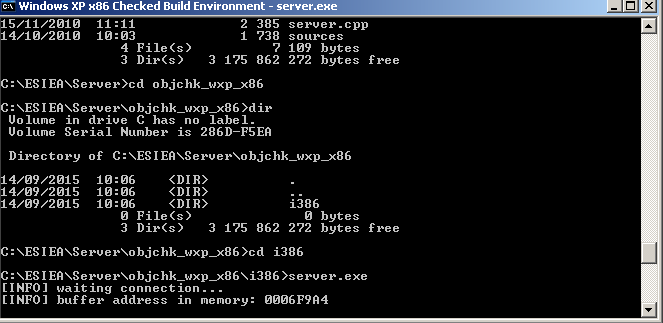
\includegraphics[width=.9\textwidth]{img/prompt1.png}
 \caption{Prompt au lancement du serveur}
\end{figure}

Soit le texte suivant :
\begin{verbatim}
  [INFO] waiting for connection...
  [INFO] buffer address in memory: 0006F9A4
\end{verbatim}
Le serveur nous signale ainsi qu'il est en attente d'une connexion client. Il nous donne aussi l'adresse mémoire du buffer, ici, \textit{0006F9A4}.

\subsection{Analyzing the server source code}

Dans le code source, il est possible de retrouver, ligne 54 et 55 l'allocation du buffer et le \textit{printf} affiché au lancement du programme serveur :
\begin{verbatim}
  char buf[BUF_SIZE];
  printf("[INFO] buffer address in memory: %p\n", buf);
\end{verbatim}
La taille du buffer étant définie par la variable \textit{BUF\_SIZE}, sa taille est donc de :
\begin{verbatim}
  #define BUF_SIZE 0x410
\end{verbatim}
Ligne 51, nous pouvons aussi retrouver le \textit{printf} du prompt signalant à l'utilisateur que le serveur est en attende d'une connexion client :
\begin{verbatim}
  printf( "[INFO] waiting connection...\n" );
\end{verbatim}
~\\
Parmi les variables et fonctions que l'on va pouvoir classer d'importantes dans le code source, nous allons pouvoir retrouver la fonction \textit{strcpy(buf, recvbuf);}. Cette dernière va permettre de copier le contenu de \textit{recvbuf} dans \textit{buf}. Le problème de cette fonction est qu'elle ne vérifie jamais si le buffer à copier n'est pas plus grand que le buffer de destination.

\subsection{Analyzing the server with WinDBG}


\begin{figure}[H]
 \centering
 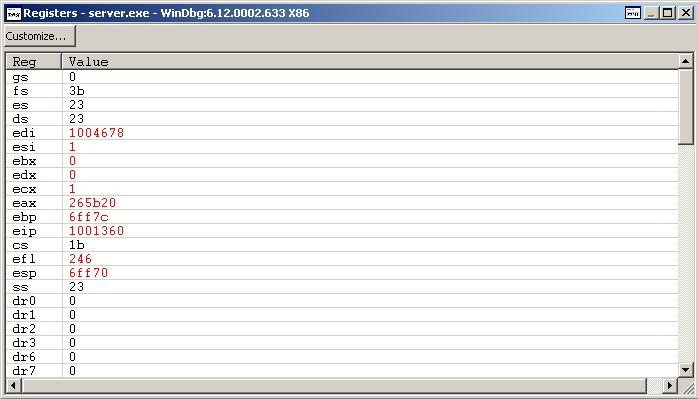
\includegraphics[width=.9\textwidth]{img/41.JPG}
 \caption{État de la mémoire au lancement du code, avant la fonction serv}
\end{figure}
On peut alors retrouver les valeurs d'\textit{esp}, \textit{ebp}, \textit{eip} :
\begin{description}
 \item[\textit{esp}] : 0006ff70
 \item[\textit{ebp}] : 0006ff7c
 \item[\textit{eip}] : 01001360
\end{description}


\begin{figure}[H]
 \centering
 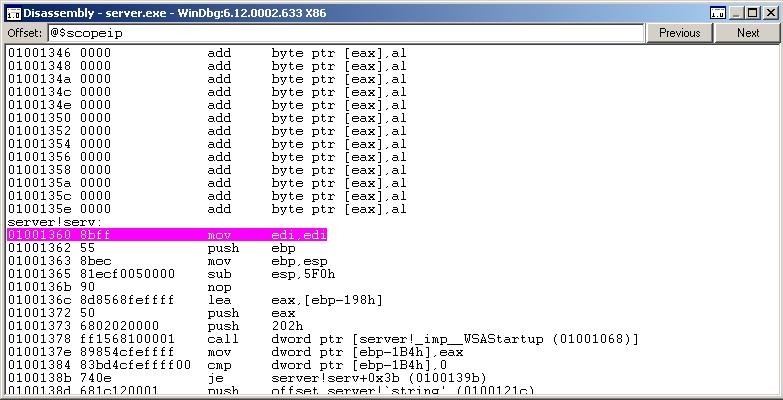
\includegraphics[width=.9\textwidth]{img/4_3.JPG}
 \caption{Liste des instructions mémoire lors de l'exécution du serveur}
 \label{img:4.3}
\end{figure}

Comme on peut le voir sur le screenshot \ref{img:4.3}, les instructions mémoire prolog destinées à la fonction \textit{serv} sont les suivantes :
\begin{verbatim}
  01001362 55              push    ebp
  01001363 8bec            mov     ebp,esp
  01001365 81ecf0050000    sub     esp,5F0h
\end{verbatim}
On retrouve ainsi les trois fonctions de la phase du prolog : \textit{push}, \textit{mov} et \textit{sub}.\\
Une fois le prolog fini, nous pouvons relever les valeurs suivantes pour \textit{esp}, \textit{ebp} et \textit{eip} :
\begin{description}
 \item[\textit{esp}] : 0006f97c
 \item[\textit{ebp}] : 0006ff6c
 \item[\textit{eip}] : 0100136b
\end{description}
\begin{figure}[H]
 \centering
 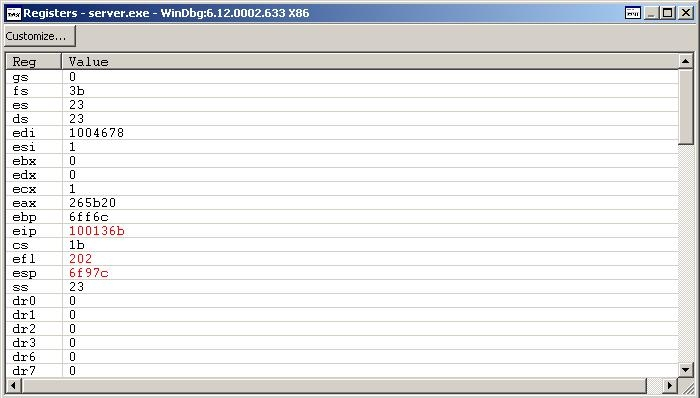
\includegraphics[width=.9\textwidth]{img/42.JPG}
 \caption{État de la mémoire après le prolog}
 \label{img:42}
\end{figure}
En regardant dans la fenêtre \textit{Memory}, nous pouvons chercher l'adresse mémoire d'\textit{ebp}. Une fois trouvé, nous pouvons chercher \textit{ebp + 4} :
\begin{figure}[H]
 \centering
 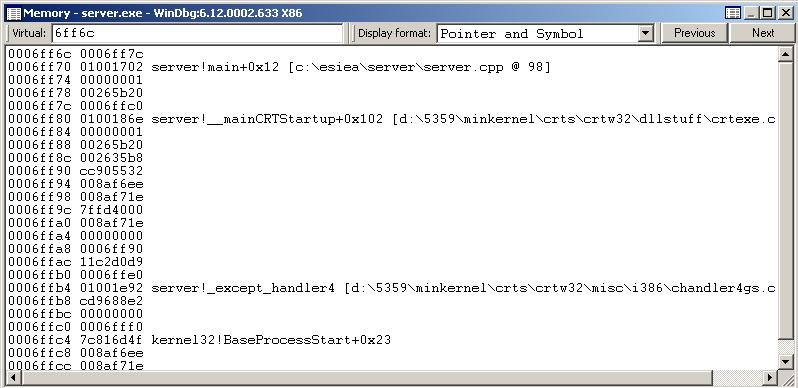
\includegraphics[width=.9\textwidth]{img/43.JPG}
 \caption{Pointer and symbol pour \textit{ebp} et \textit{ebp + 4}}
 \label{img:43}
\end{figure}
On remarque alors qu'à l'adresse mémoire \textit{ebp + 4} (6ff70), nous allons retrouver la fonction \textit{main} du programme serveur (\textit{server!main}). Cet espace mémoire s'étend jusqu'à l'espace mémoire 1001702.\\
En regardant dans la fenêtre \textit{Disassembly}, il est possible de rentrer l'espace mémoire 1001702 et remarquer que cela correspond à l'epilog. En effet, en regardant les appels assembleurs, nous pouvons remarquer que l'on a un \textit{pop} d'\textit{ebp} (adresse mémoire 1001704) suivi d'un \textit{ret} (adresse mémoire 1001705). Ce dernier va alors retourner dans la pile mémoire du \textit{main} en quittant celle de la fonction \textit{serv}.
\begin{figure}[H]
 \centering
 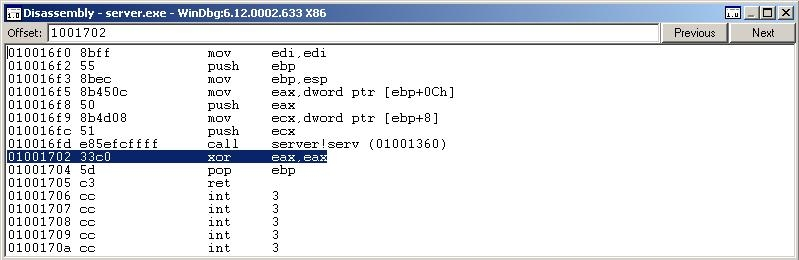
\includegraphics[width=.9\textwidth]{img/44.JPG}
 \caption{Adresse mémoire de l'\textit{epilog}}
 \label{img:44}
\end{figure}
~\\
Afin de trouver l'\textit{upper bound} du buffer que nous devons injecter afin de réécrire la valeur de \textit{ret}, nous devons prendre la quantité d'information contenue entre \textit{ebp} et \textit{esp}. Nous savons aussi que nous avons deux adresses codées sous 4 octets (\textit{SAVED EBF} et \textit{SAVED EIP (ret)}). Ainsi, nous retrouvons la formule suivante :
\begin{displaymath}
 \textit{EBP}-\textit{ESP}+4+4=6FF6C-6F97C+4+4=5F8
\end{displaymath}
\\~\\
En parcourant le code avec le debugger et en utilisant la fenêtre \textit{Disassembly}, nous pouvons retrouver l'allocation mémoire en assembleur du buffer cible.
\begin{figure}[H]
 \centering
 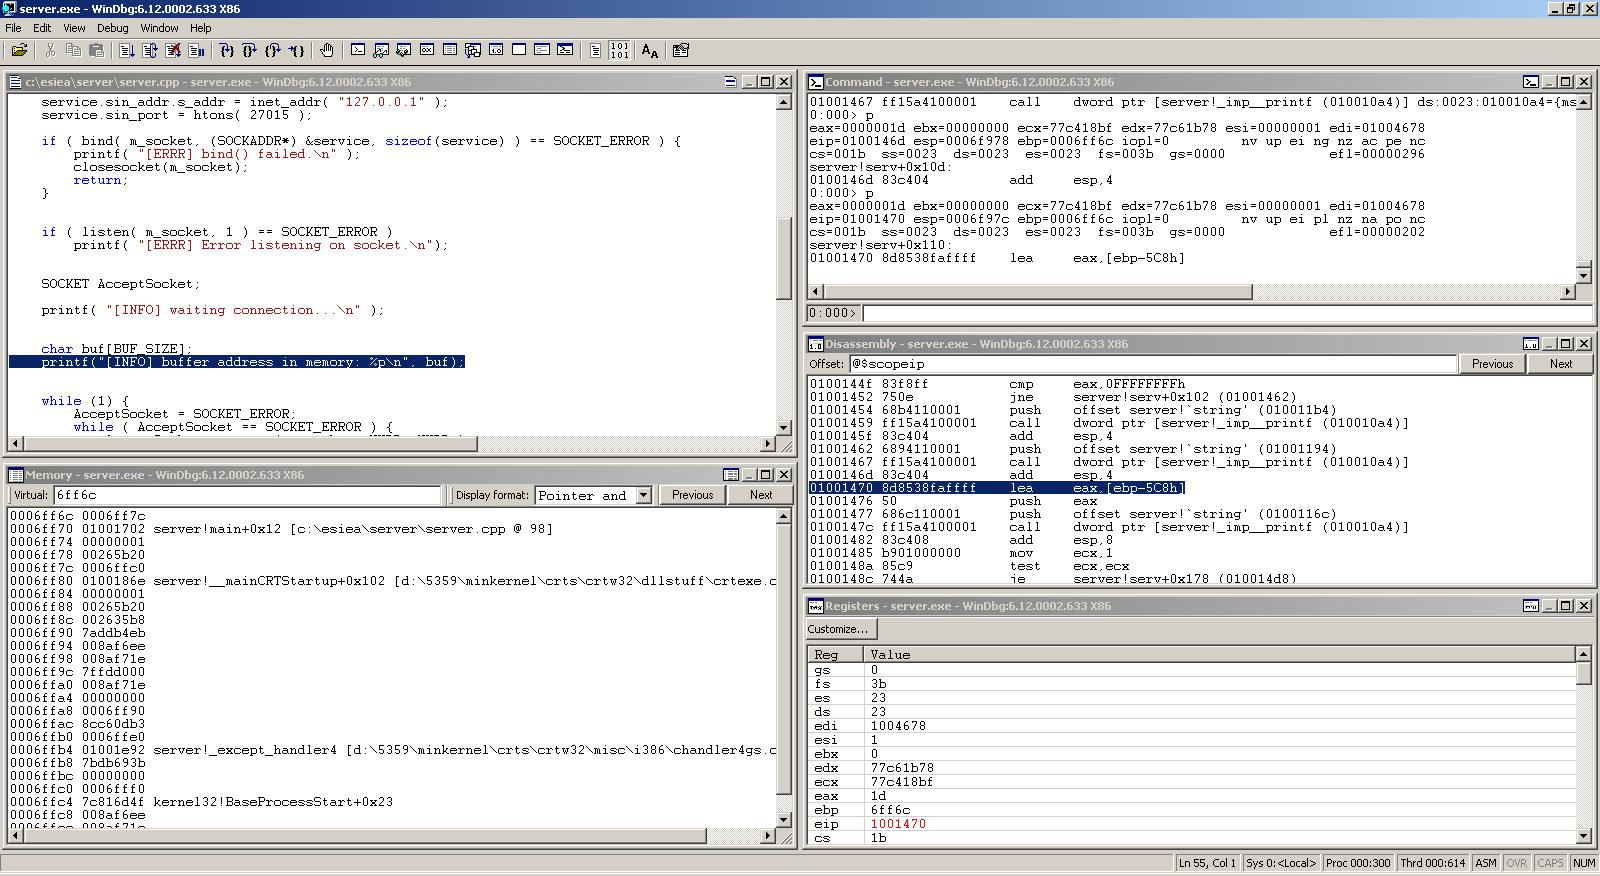
\includegraphics[width=.9\textwidth]{img/46.JPG}
 \caption{Adresse mémoire du buffer cible}
 \label{img:46}
\end{figure}
Nous pouvons voir sur le screenshot \ref{img:46} que ce dernier est alloué à partir de l'espace mémoire \textit{ebp-5C8}.\\
Ainsi, en reprenant la définition de la pile, nous savons que :
\begin{itemize}
 \item Le buffer cible s'arrête à l'adresse \textit{ebp-5C8}
 \item Nous pouvons retrouver deux variables avant notre buffer
 \begin{itemize}
  \item Saved \textit{ebp}
  \item Saved \textit{eip} (ret)
 \end{itemize}
  Or ces deux variables sont enregistrées sur 4 octets chacune.
\end{itemize}
Ainsi, nous pouvons en déduire que pour réécrire sur la valeur de ret, nous devons envoyer un buffer jusqu'à $ebp-5D0$. Soit un buffer d'une taille de $1488$ octets.